cis- and trans-Pyrenes have been deposited on h-BN/Cu(111).
One can easily discern single molecules in an array of many, little to no contamination is visible.

Spectra have been taken and may be compared to those of Tobias Hoh (Ba-thesis). Units cells are developed.

%%%%%%%%%%%%%%%%%%%%%%%%%%%%%%%%% Pyrene-files
%%%%%%% Measured Juni '16
%%%%%%%%%%%%%%%%%%%%%%%%%%%%%%%%%%%%% Cis-pyrenes on h-BN /Cu(111)
\paragraph {cis-pyrenes}
Binding motivs of cis-pyrene include dense packed islands that grow in distinct directions. 
\begin{figure}[!h]
\centering
% another image is 
%  \includegraphics[width=0.3\textwidth]{./images/F160624.172817-model}
 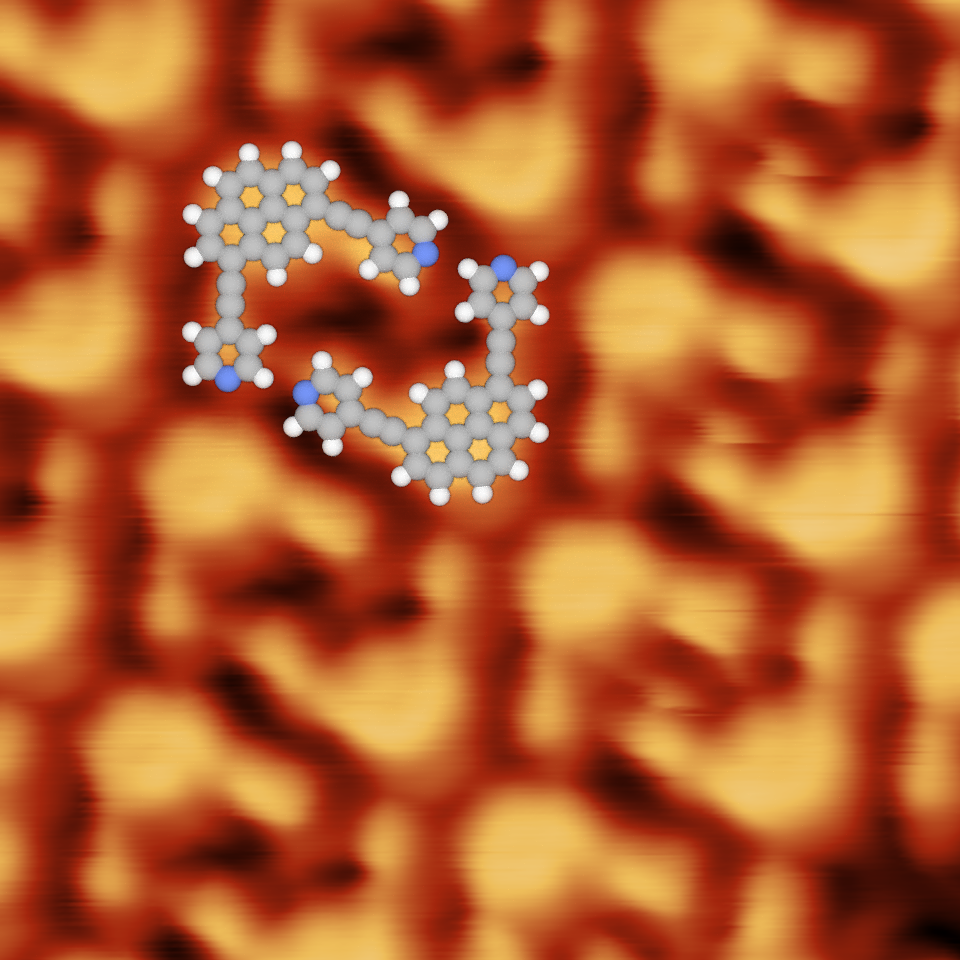
\includegraphics[height=0.45\textwidth]{./images/F160624-182952-model.png}
 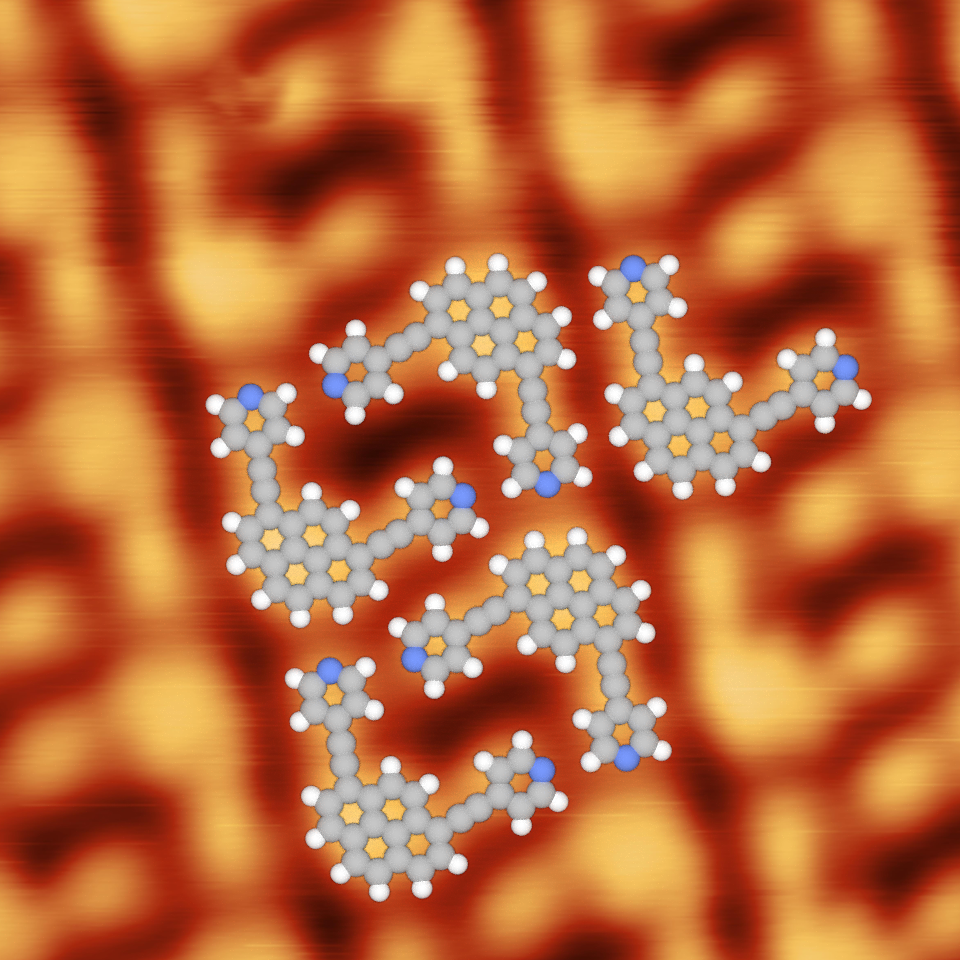
\includegraphics[height=0.45\textwidth]{./images/F160624-171335-model.png}
 \caption{Molecules adsorbed on h-BN/Cu(111) at room temperature form a rectangular unit cell with lattice vectors having a lenght of $a_1 = \SI{1.47}{\nano \meter}$ and $a_2 = \SI{2.13}{\nano \meter}$ respectively. The functionalized end of the leg may never point straight to another functionalized leg's end (the nitrogen), but rather slightly apart (to an H-atom). Images are both 5.5 x 5.5 nm in size}
\end{figure}

Some islands (like the one shown in figure \ref{fig:cis-stripe}show clear evidence of preferred growth direction. The pyrenes are not affected in their orientation or arrangement by the h-BN. Their binding motiv is driven by the fact that the nitrogen-terminated legs will favour to form hydrogen bridges to neighboured molecules (their H-atoms) instead of facing another nitrogen.

\begin{figure}[!h]
\centering
 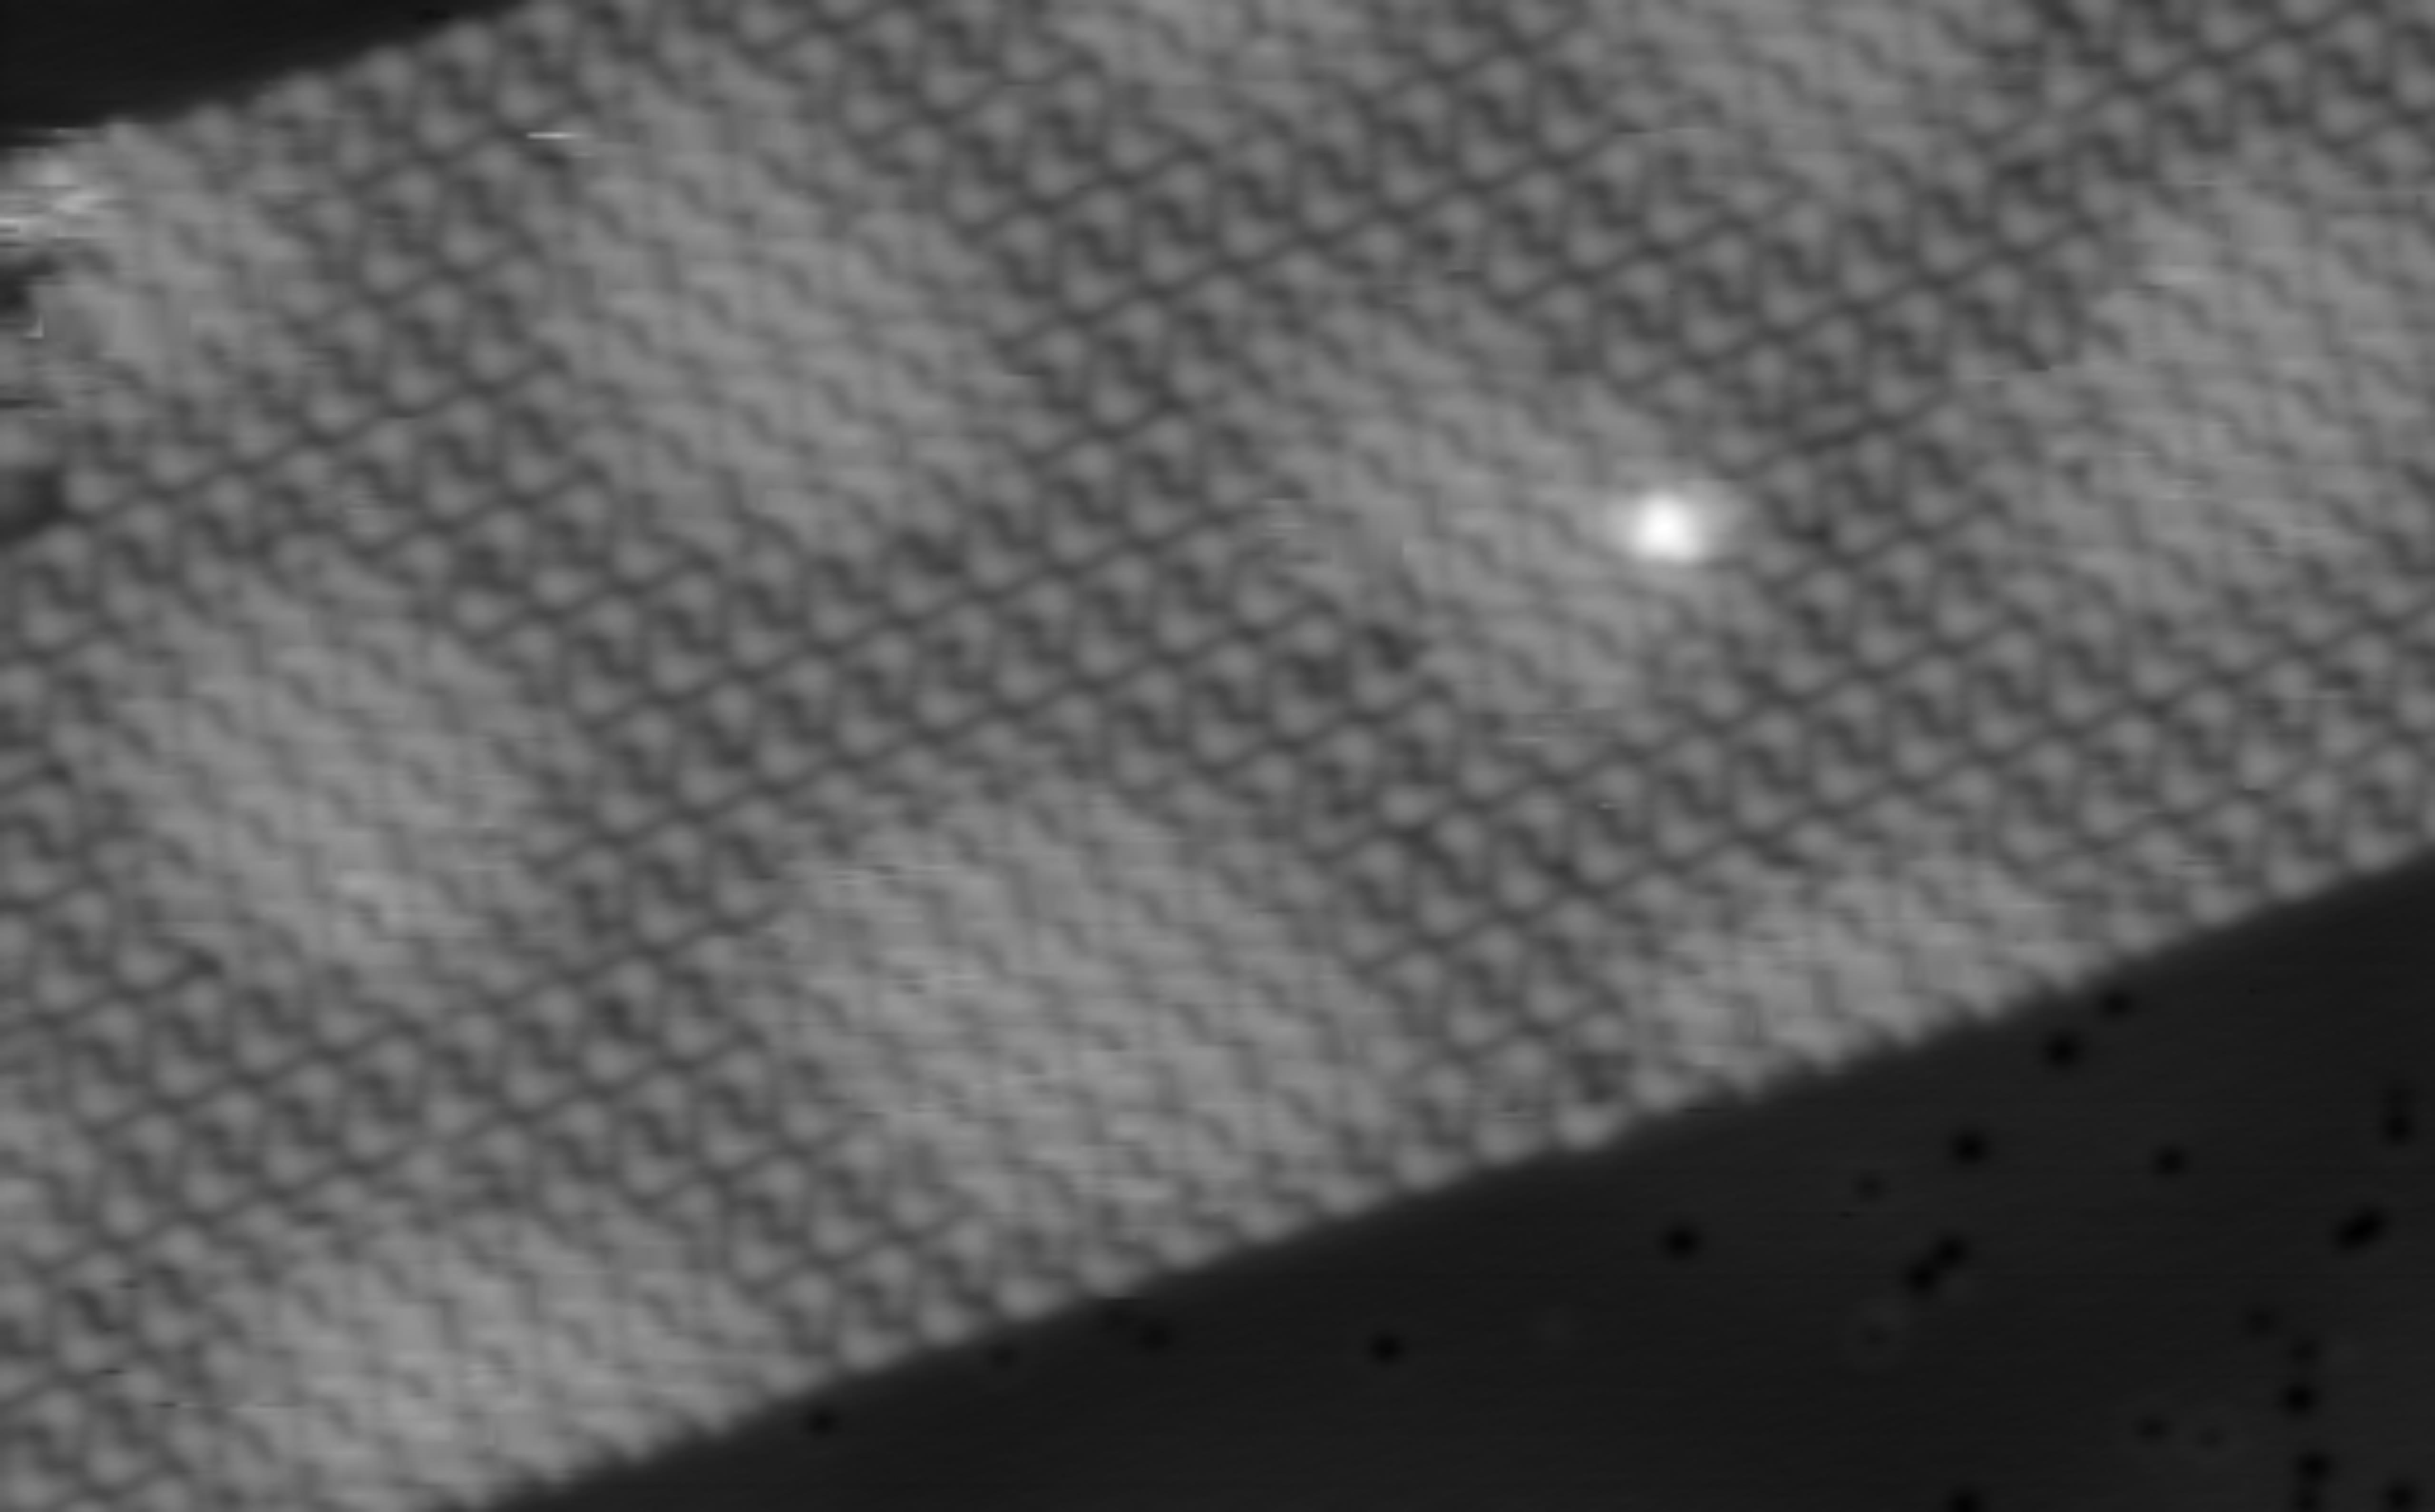
\includegraphics[height=0.35\textwidth]{./images/F160627-103358.png}
 \caption{Elongated island of cis-pyrene on h-BN/Cu(111). The moire is visible as brighter protrusions. Islands exhibit larger perimeter along $a_1$ than $a_2$ which may indicate a stronger binding along this direction.} 
\label{fig:cis-stripe}
\end{figure}

The introduced h-BN layer electronically decoupled the molecules. From time to time, resolution of the frontier orbitals could be achieved (figure \ref{fig:cis-orbital}). Calculations have been done.\footnote{molecule was geometrically optimized and afterwards the orbitals have been calculated with the gaussian package - recalculate because no license available... TD-SCF-DFT method with MPW1PW91 functional with a 6-311G basis set}

A close look shows the same pattern of orbitals experimentally observed when compared to the theoretical result. Resolution of the HOMO state could not be achieved.

\begin{figure}[!h]
\centering
 \subfigure[STM image]{
 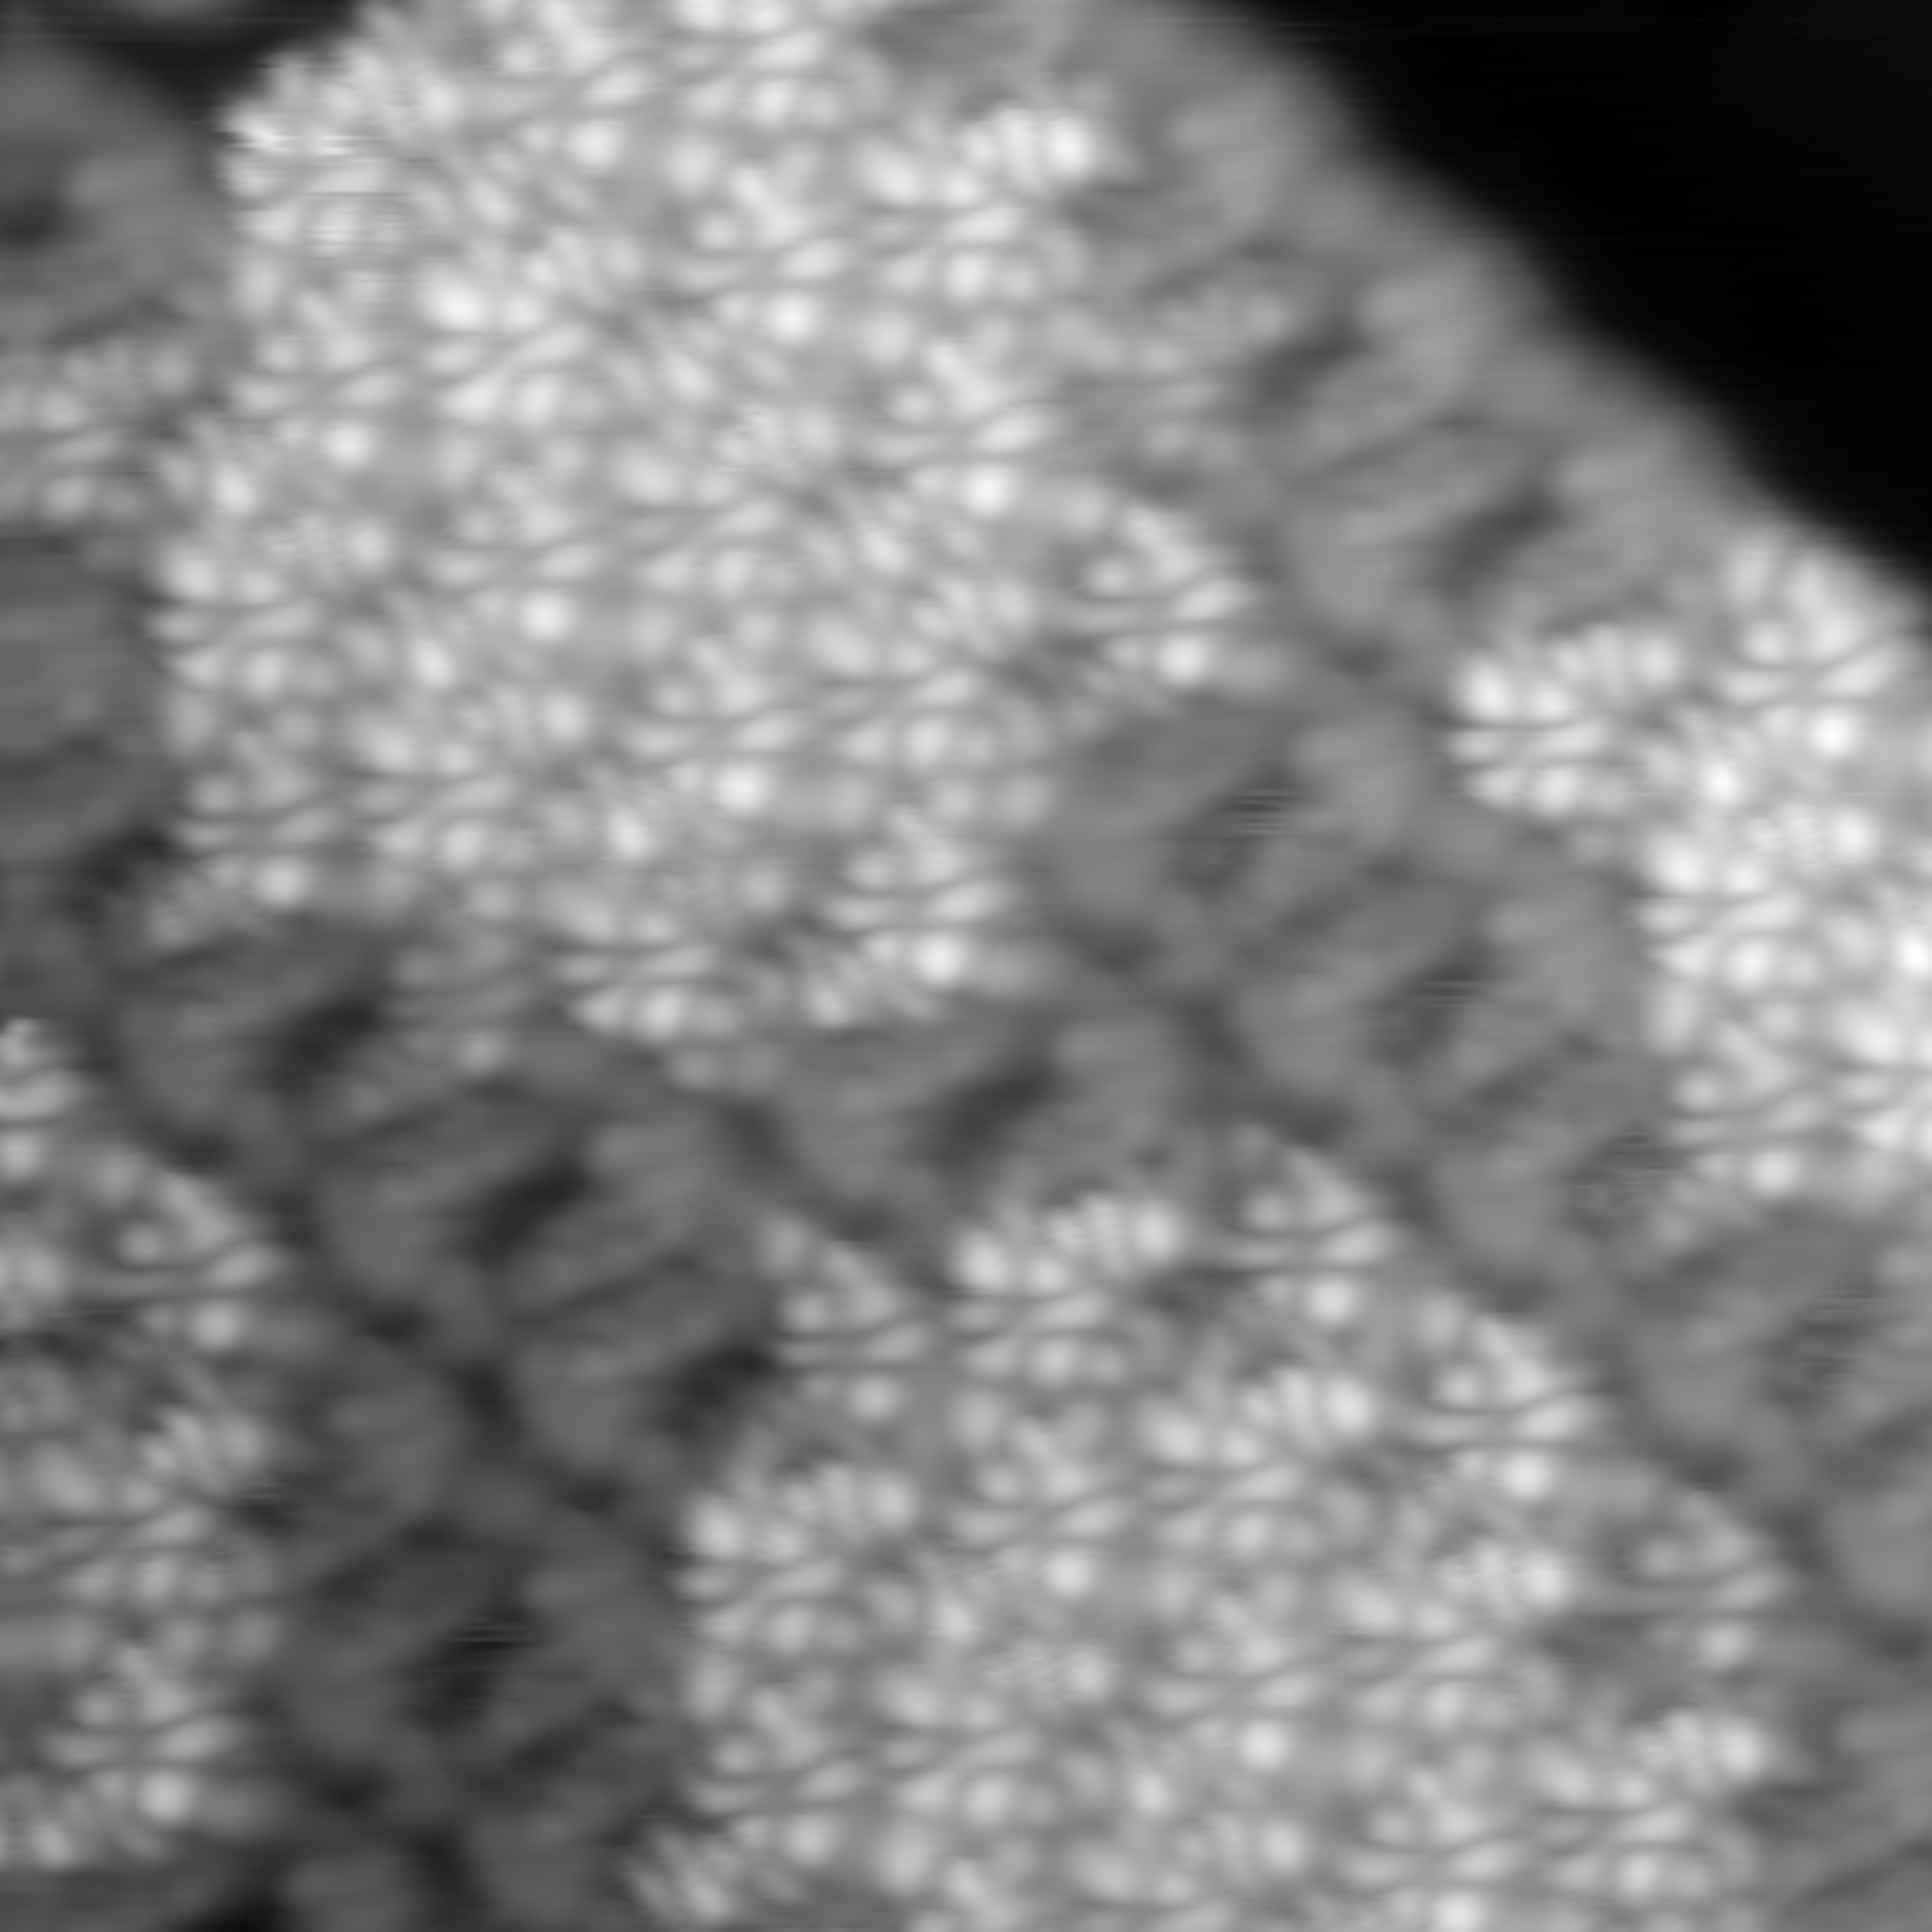
\includegraphics[width=0.45\textwidth]{./images/F160627-155029.png}
 }
 \subfigure[DFT calculated orbital arrangement]{
 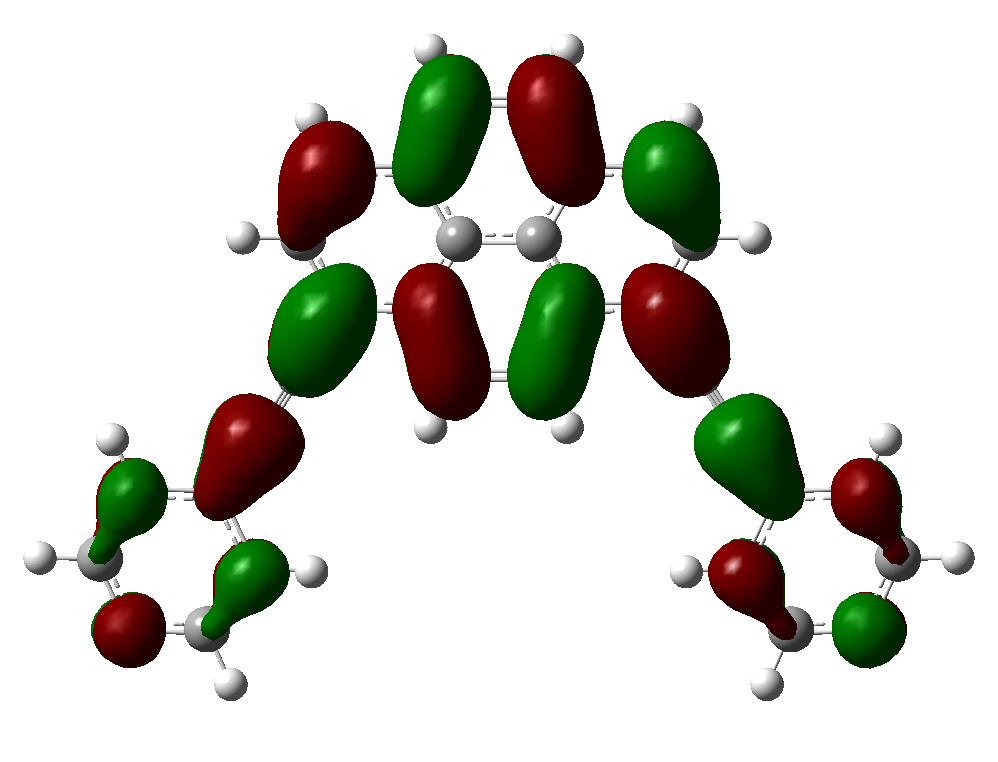
\includegraphics[angle=90,width=0.35\textwidth]{./images/cis-lumo-top.jpg}
 }
 \subfigure[Comparison to already measured tetra-pyrene/h-BN/Cu(111) at \SI{1.4}{\V}]{
 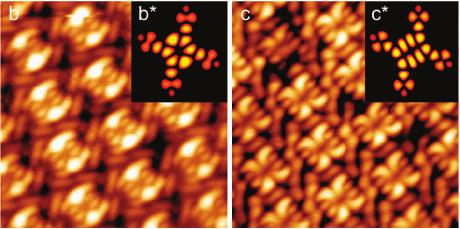
\includegraphics[width=0.8\textwidth]{./images/Tobias-Hoh-Ba-tetra-pyrene-orbitals.jpg}
 }
\caption{Molecular orbitals of cis-pyrene on h-BN/Cu(111) - a) shows a STM image recorded ($U_b=\SI{1.5}{\V}$) next to the LUMO-state of the molecule , b) shows the calculated LUMO. c) reproduced graphic from Tobias Hoh's Ba-thesis} 
\label{fig:cis-orbital}
\end{figure}
A similar molecule (tetra-pyrene) has been investigated (see Tobias Hoh Ba-thesis) on h-BN/Cu(111) with similar results. They show a similar pattern (with four legs of course). 

Electronic properties have been studied by means of STS.

\begin{figure}[!h]
\centering
 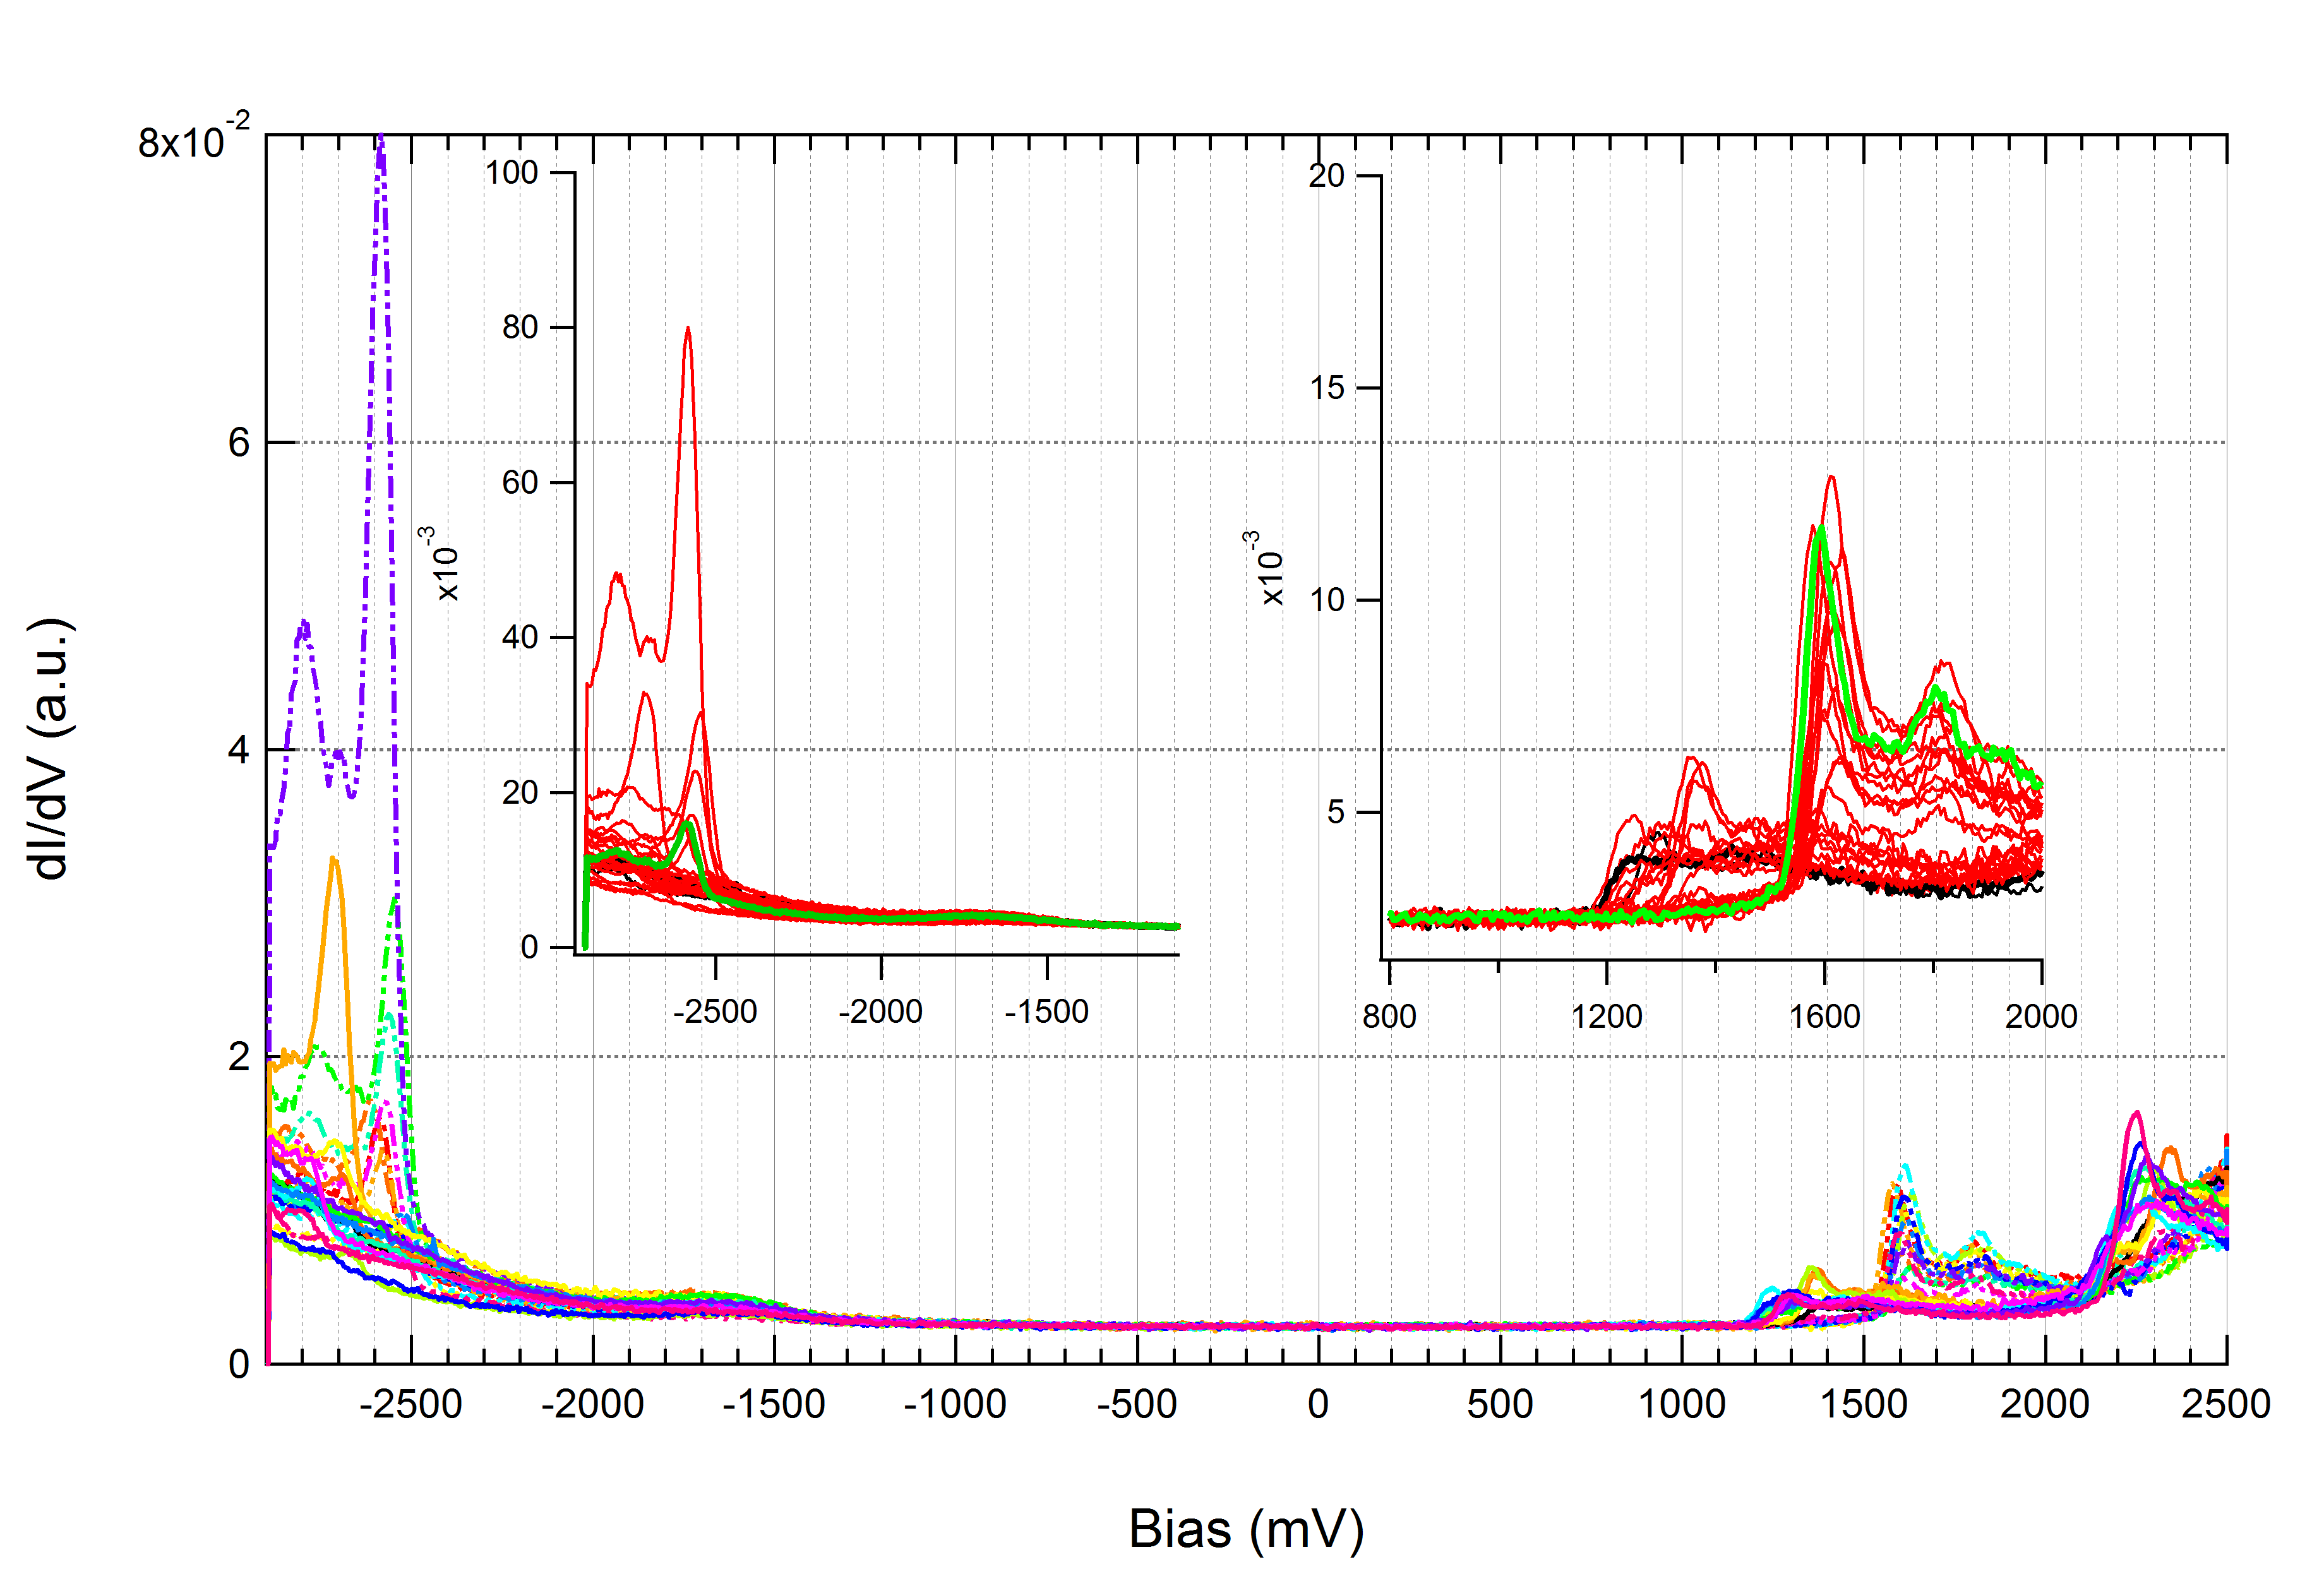
\includegraphics[width=0.9\textwidth]{./images/spectra-in-moire.png}
 \caption{Scanning tunneling spectroscopy of cis-pyrenes adsorbed on h-BN/Cu(111). Insets show enlarged HOMO/LUMO regions. Black spectra is taken on  hill-, green spectra is taken in valley-regions of the moire. In between a continous shift is observed.} 
\label{fig:cis-orbital}
\end{figure}


\paragraph {cis-pyrenes / trans-pyrenes}
%%%%%%%%%%%%%%%%%%%%%%%%%%%%%%%%%%%%% Cis-pyrenes | Trans-pyrenes on h-BN /Cu(111)
A mixture of both species has been deposited too. When trans-pyrenes are evaporated onto the sample with cis-pyrenes already deposited, following motivs show up. The local density of molecules induces different binding motivs depending on the position on the sample. Different areas of different packing densities are observed, which show different tesselation. 
\begin{itemize}
\item The first motiv looks like a kagome-lattice, sometimes cis-pyrenes are incorporated into this network. Their orientation within the kagome-lattice varies but their legs are always parallel to the enclosing trans-pyrenes (resulting in 6 possible positions). The kagome lattice vectors are $a_1 = a_2 = \SI{2.7(1)}{\nano \meter}$ enclosing an angle of \SI{60}{\degree}. The unit cell also consists of three molecules - one fully counted in its center and four counted half because they overlap with the neighbouring unit cell (Fig.\ref{pic:1+2} left).
\item The second motiv is more of the dense packed cis-pyrene appearance with rows of trans-pyrenes introduced between every row. This happens in a way that the cis-pyrenes are only allowed to touch nestedly. Each row extends along a certain direction, maybe induced by the affinity for the functional ends of the legs to touch the pyrene-center of the neighbouring molecule (as it is the case for the kagome lattice). The unit cell consists of 3 molecules. Two of them are cis-pyrens surrounded by 4 trans-pyrenes, which are equally shared of the adjacent unit cells thus counting only partially. Lattice vectors are  $a_1 = a_2 = \SI{2.0(1)}{\nano \meter}$ respectively enclosing an angle of \SI{75}{\degree}(Fig.\ref{pic:1+2} right).
\end{itemize}

\begin{figure}[!h]
\centering
 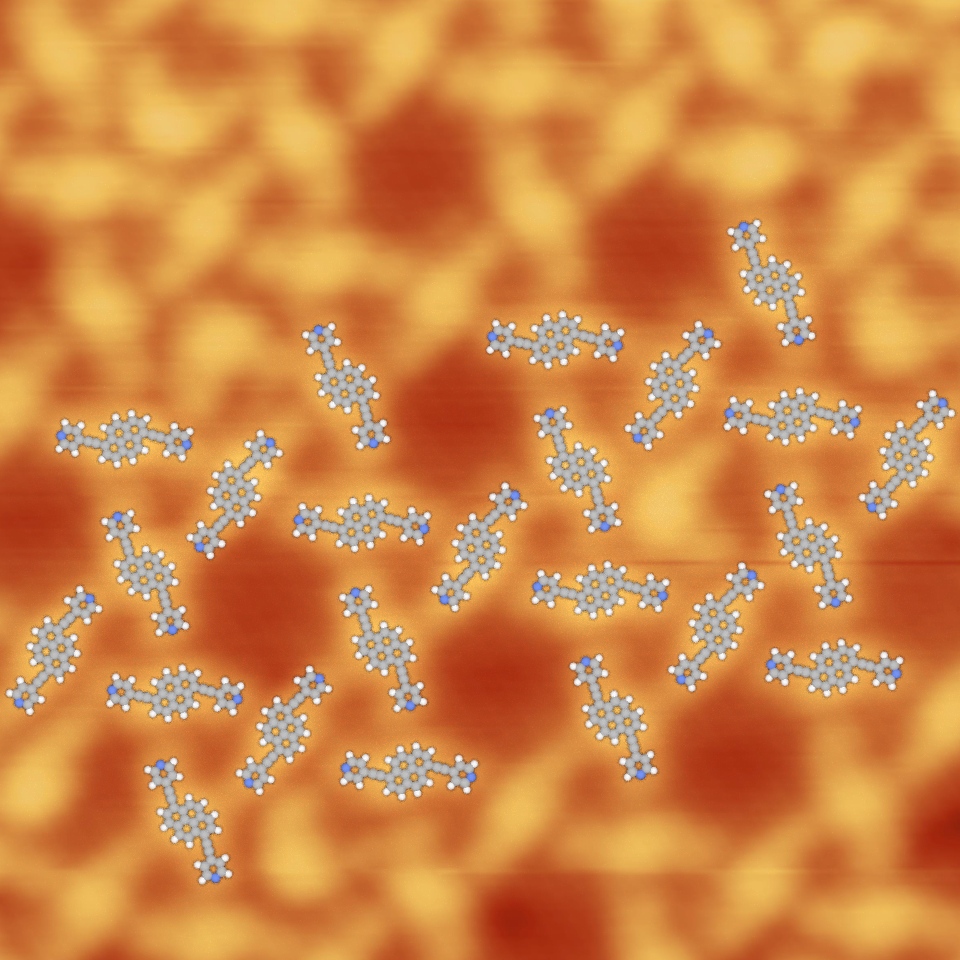
\includegraphics[height=0.4\textwidth]{./images/F160628-143559-model.png}
 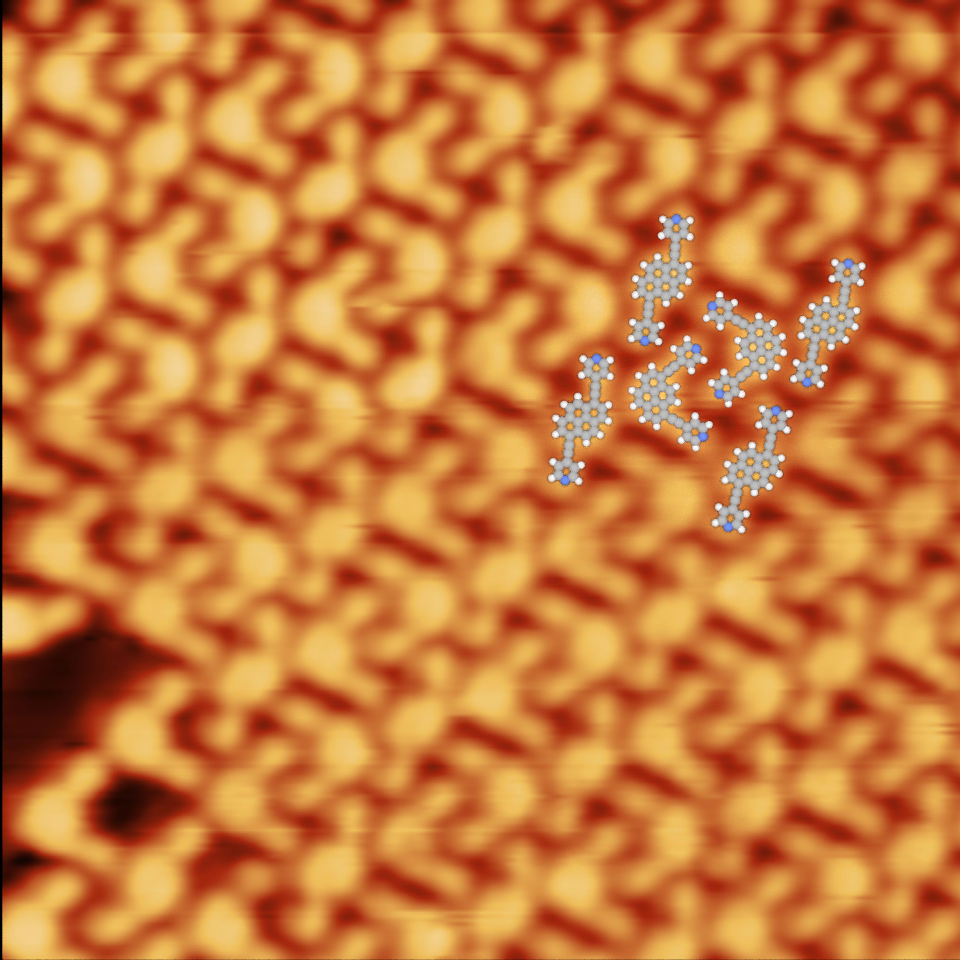
\includegraphics[height=0.4\textwidth]{./images/F160628-163557-model.png}
 \caption{Two different motivs are observed during the same preparation. One is dominantly kagome-type with cis-pyrenes trapped in their respective centers, while the other is dense packed with the trans molecules lying between the rows of cis-pyrene} 
\label{pic:1+2}
 \end{figure}

 %%%%%%%%%%%%%%%%%%%%%%%%%%%%%%%%%%%%% Trans-pyrenes
\paragraph {trans-pyrenes}
Trans-pyrene also forms dense packed islands and kogome-like areas are observed. Due to the chirality of the molecule, two types of kagome form.

When trans-pyrenes are evaporated solely onto the h-BN/Cu(111) sample two chiral motivs emerge. They are driven by the geometry of the molecules. Trans-pyrene is a chiral molecule, thus able to form chiral structures on the surface. Interestingly these chiral domains only consist of molecules with the same chiral orientation. Both domains are seperated by an unordered regime where both motivs blend. The driving force for building the kagome lattice seems to be (again) the strong interaction of the functionalized leg with the pyrene body. 

The unit cell on the left is rotated by \SI{20}{\degree} with respect to the right.

\begin{figure}[!h]
 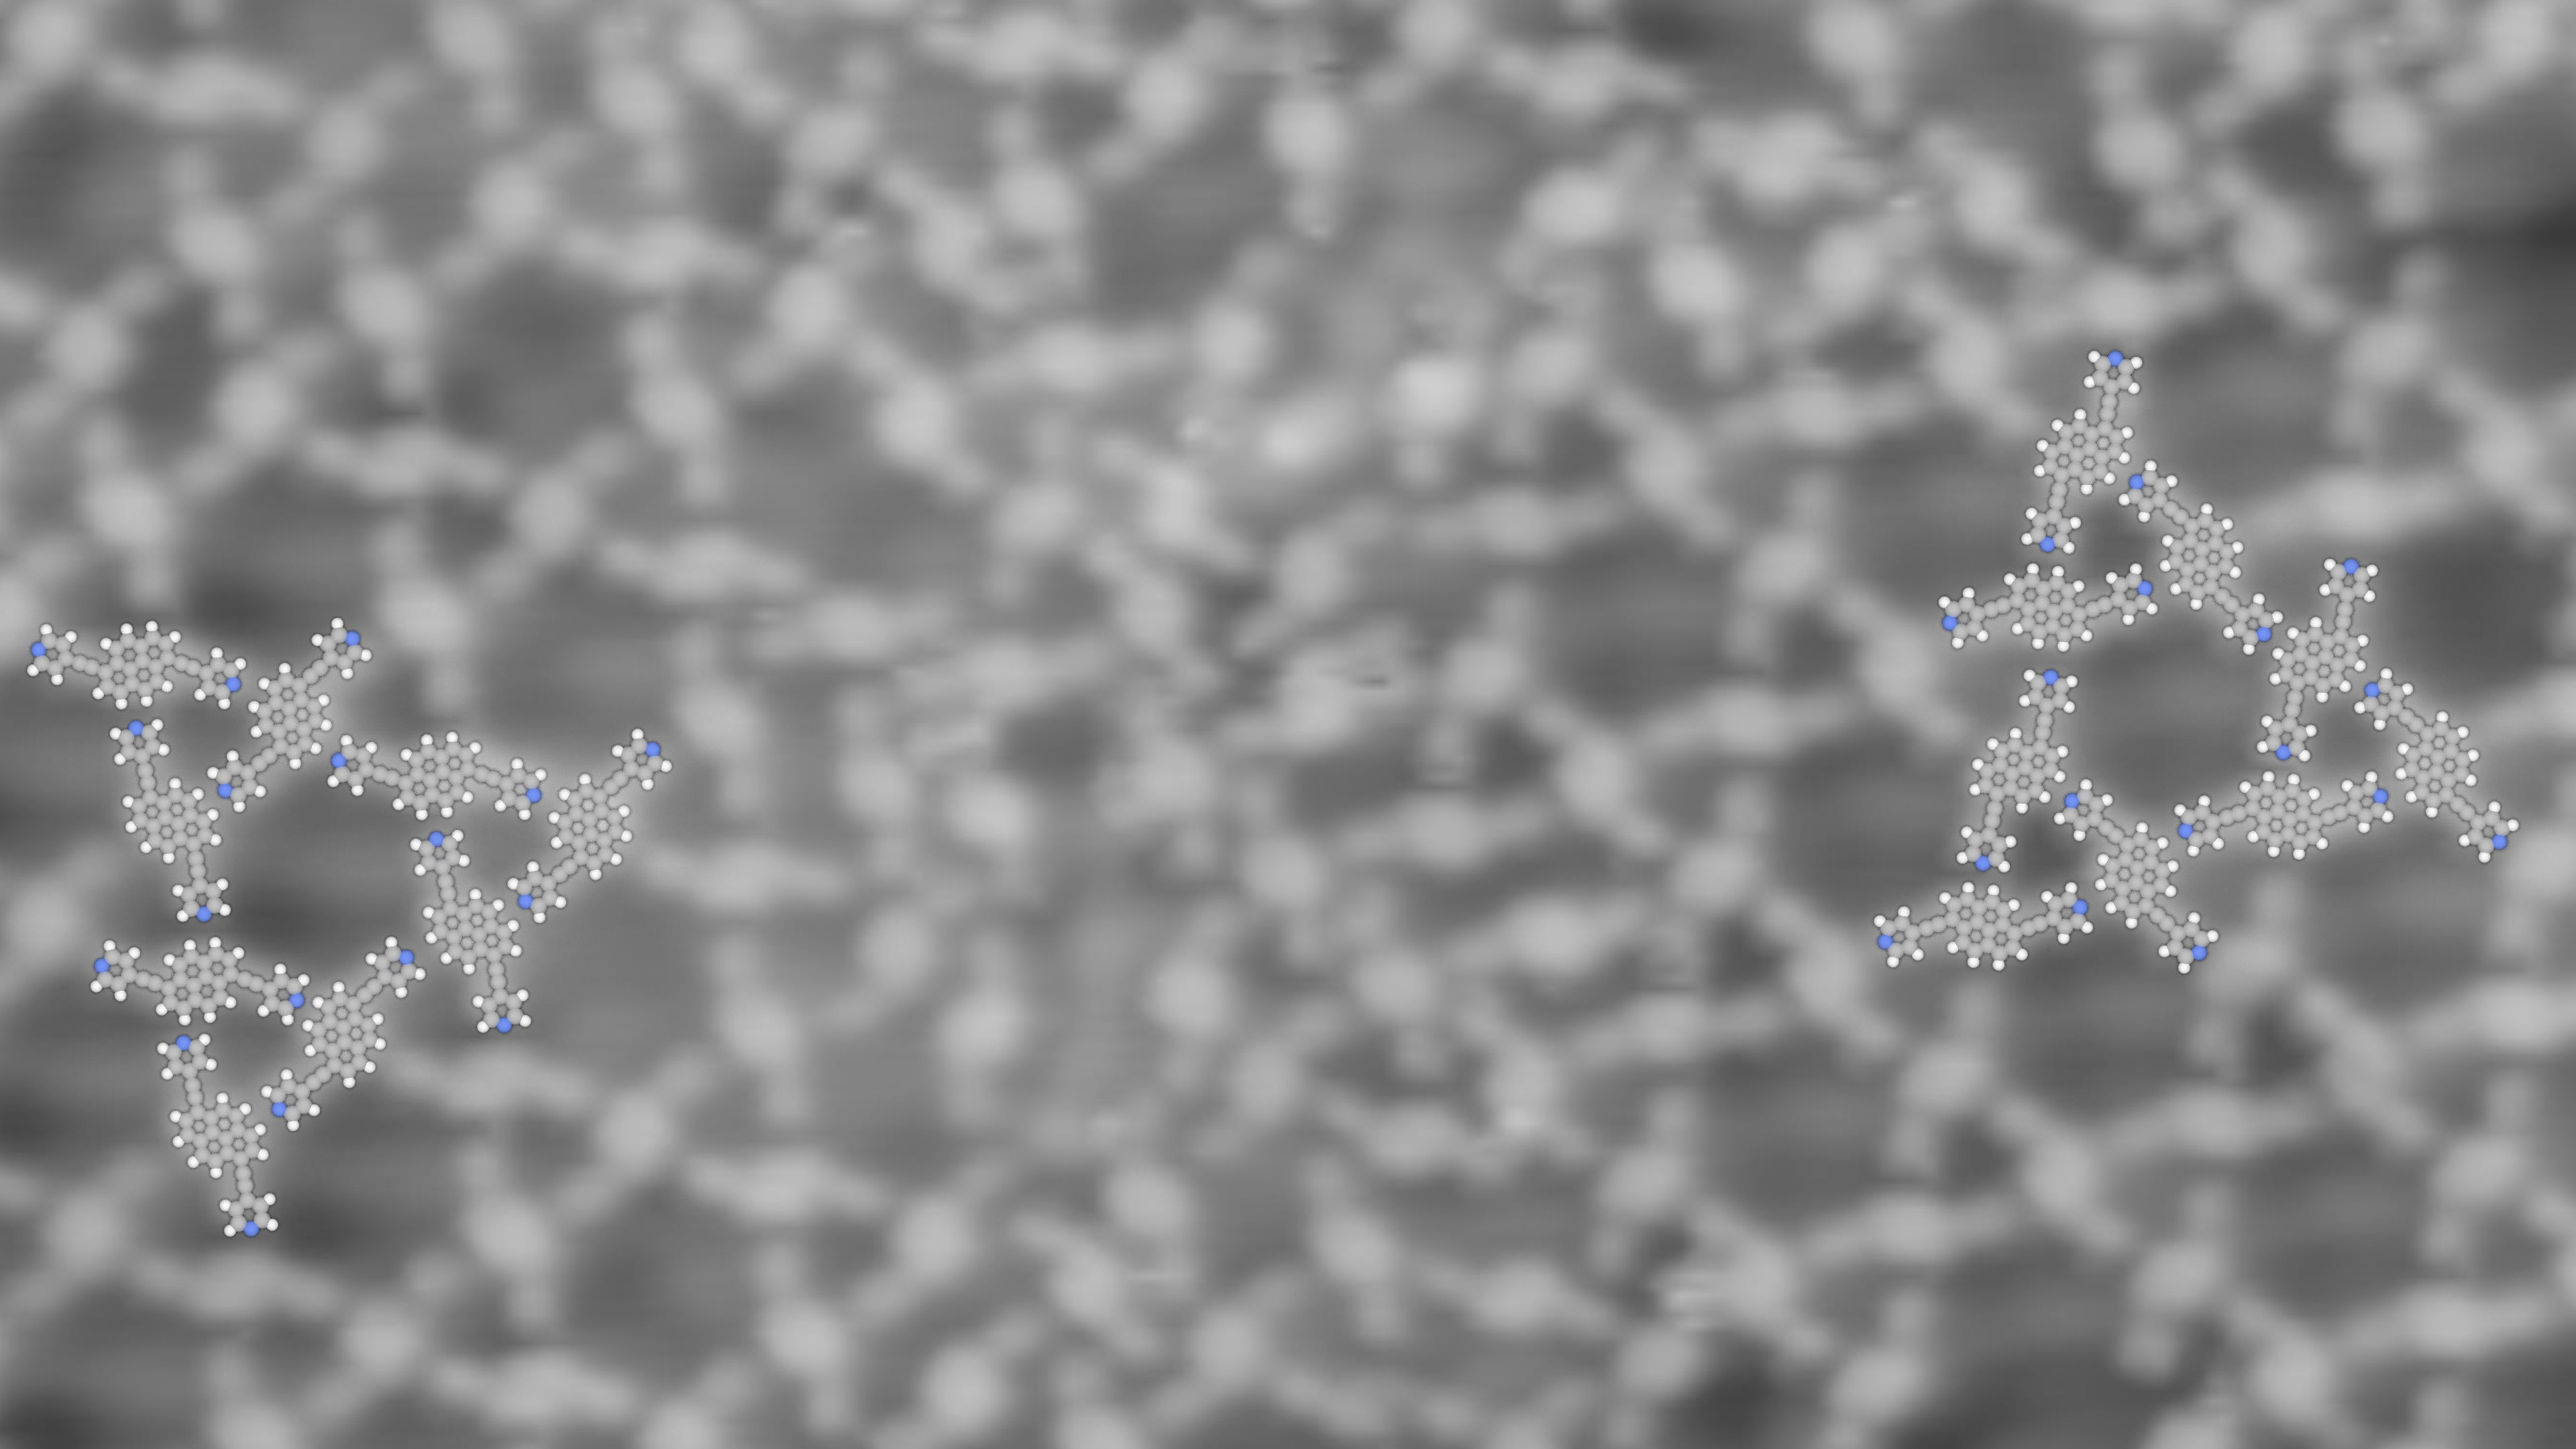
\includegraphics[width=\textwidth]{./images/F160703-143204-model.png}
  \caption{Here one can nicely see the chirality in the two domains (left/right part of the image) which is introduced by the molecular chirality itself. Length of lattice vectors are the same as for the above metioned kagome lattice(within the error margin).}
  \label{fig:trans-kagome-chiral}
\end{figure}

Two different binding motivs occure, namely the kagome trans-pyrene pattern in image \ref{fig:trans-kagome-chiral} and a dense packed pattern depicted in figure \ref{fig:trans-dense-packed}. Within this pattern one can deduce on lattice constant of \SI{2.12}{\nm} x \SI{1.4}{\nm} with an angle of \SI{145(35)}{\degree} between its lattice vectors.

\begin{figure}[!h]
\subfigure[coexisting motivs]{
 \includegraphics[width=0.9\textwidth]{./images/F160630-100625.png}}
\subfigure[dense packed motiv \SI{5.5}{\nm} x \SI{5.5}{\nm}]{
 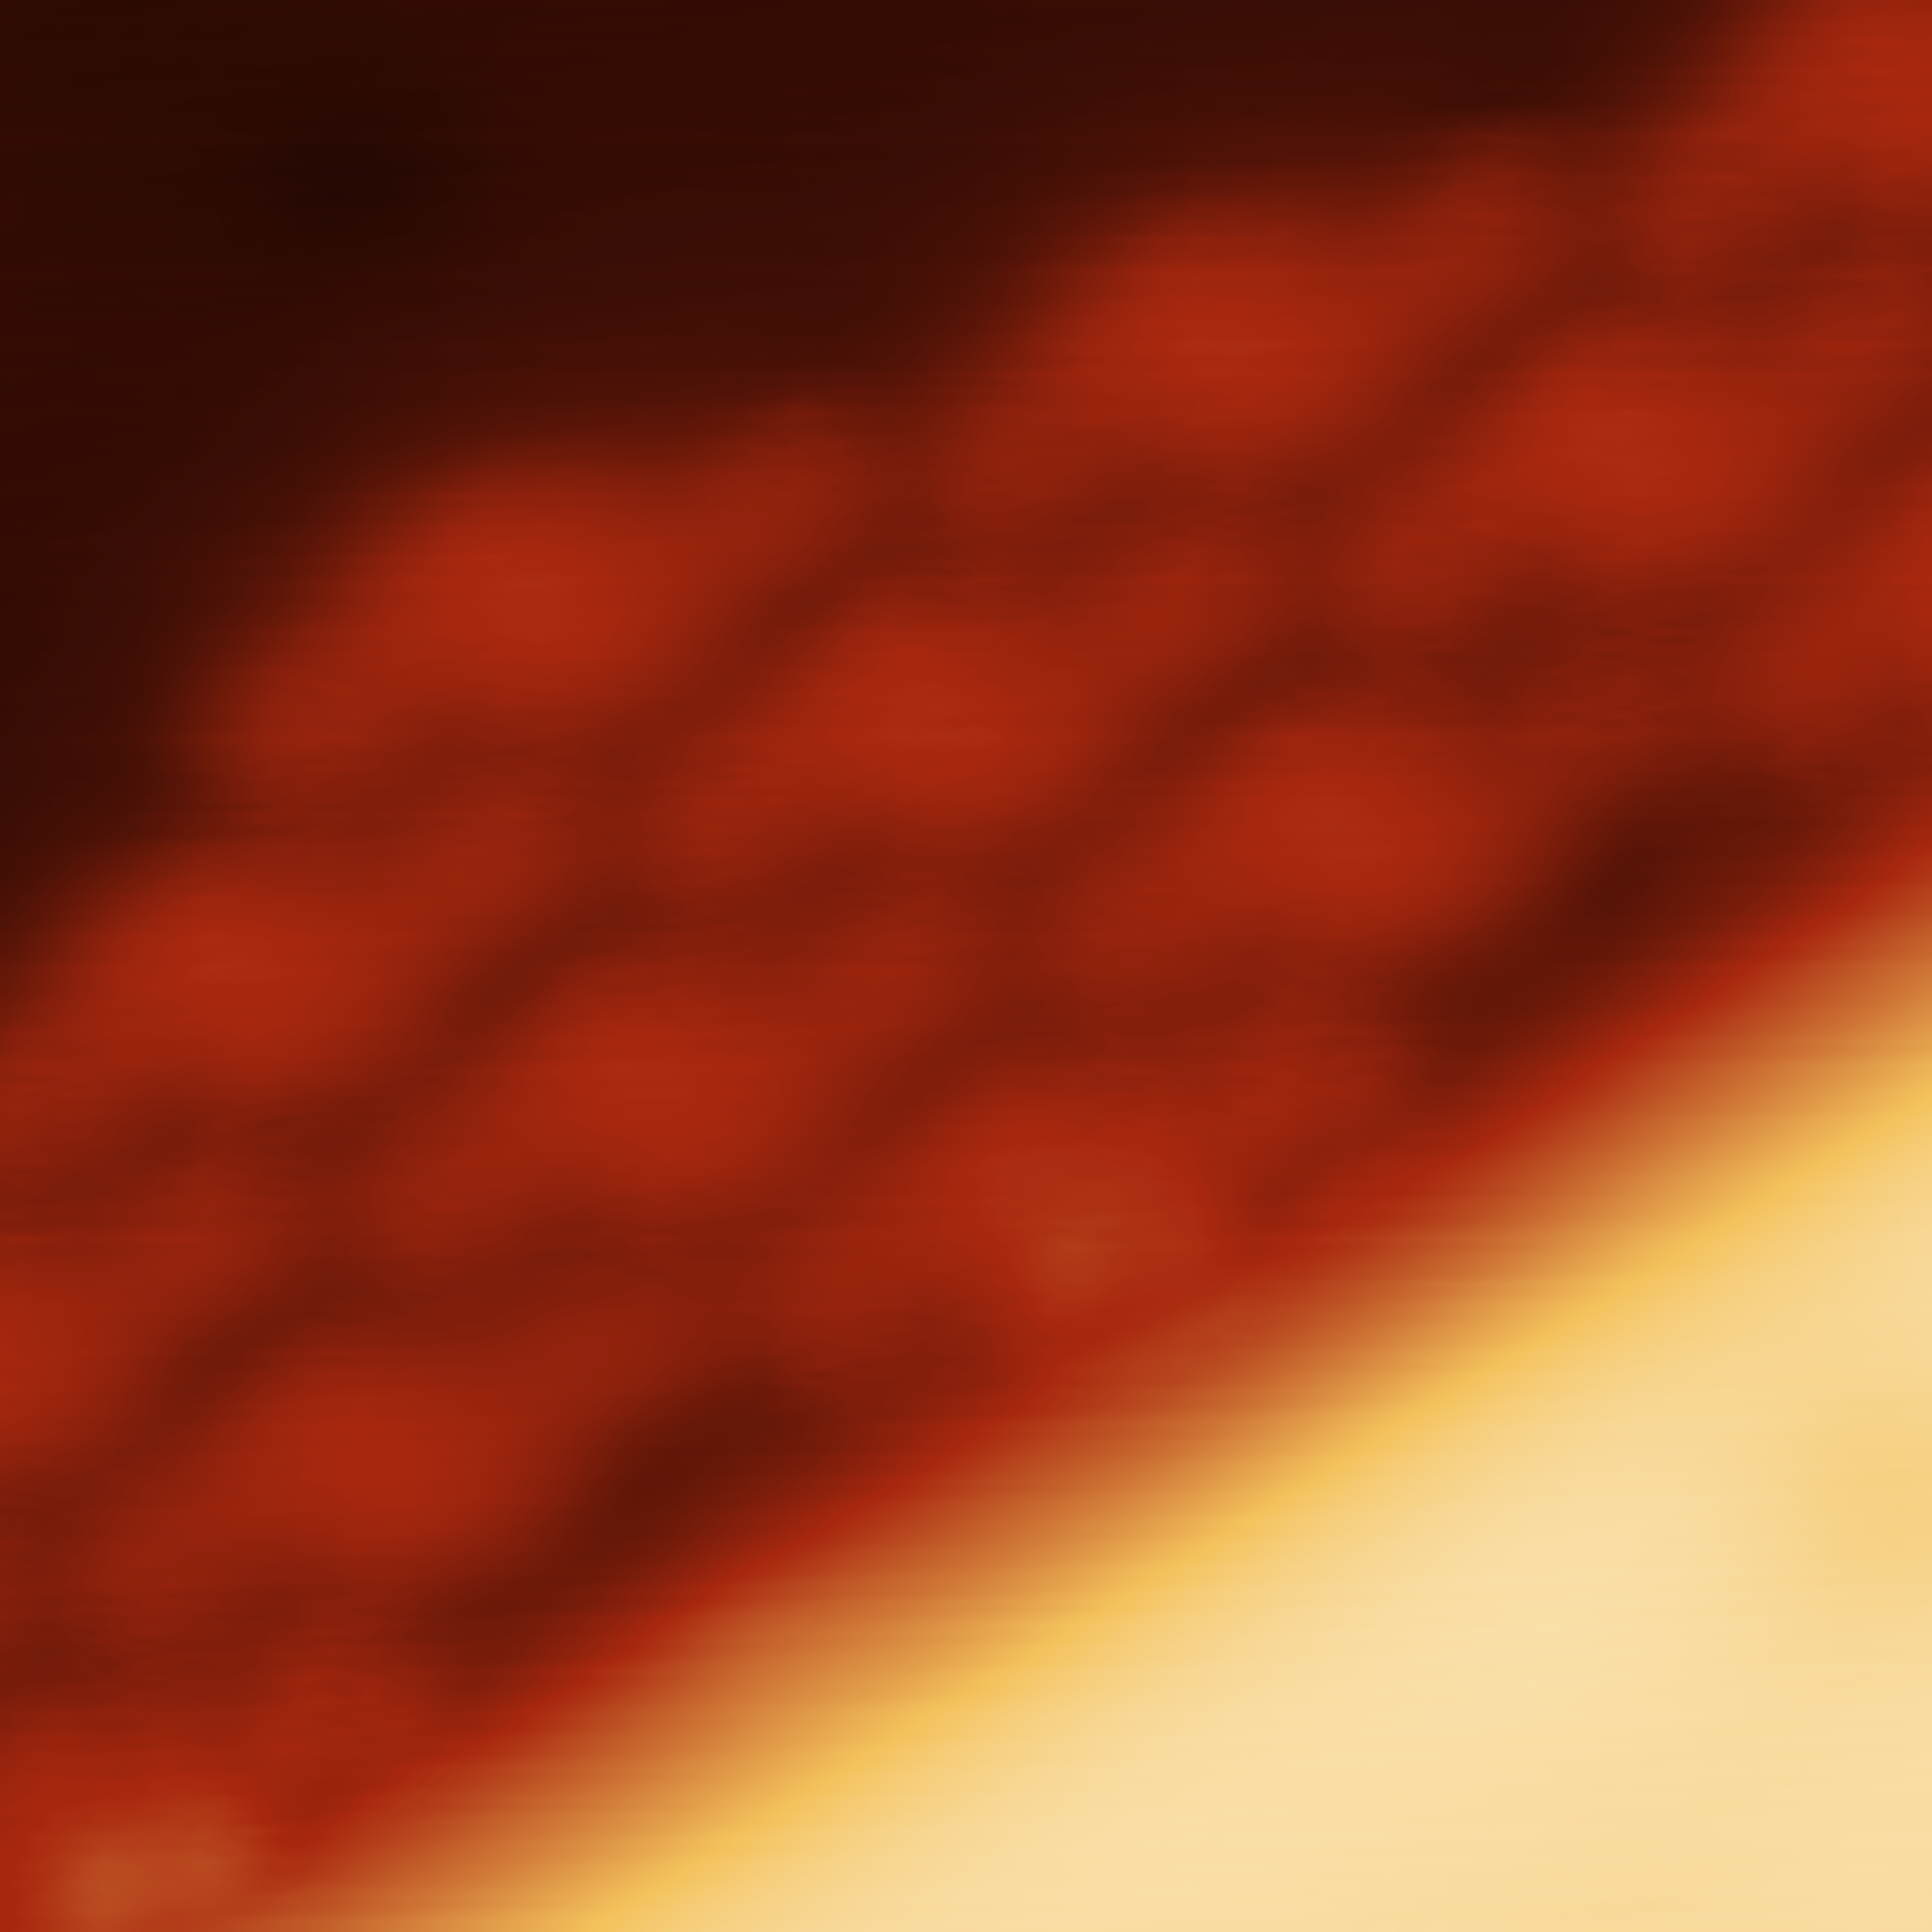
\includegraphics[width=0.45\textwidth]{./images/F160630-101110.png}}
 \subfigure[model overlayer]{
 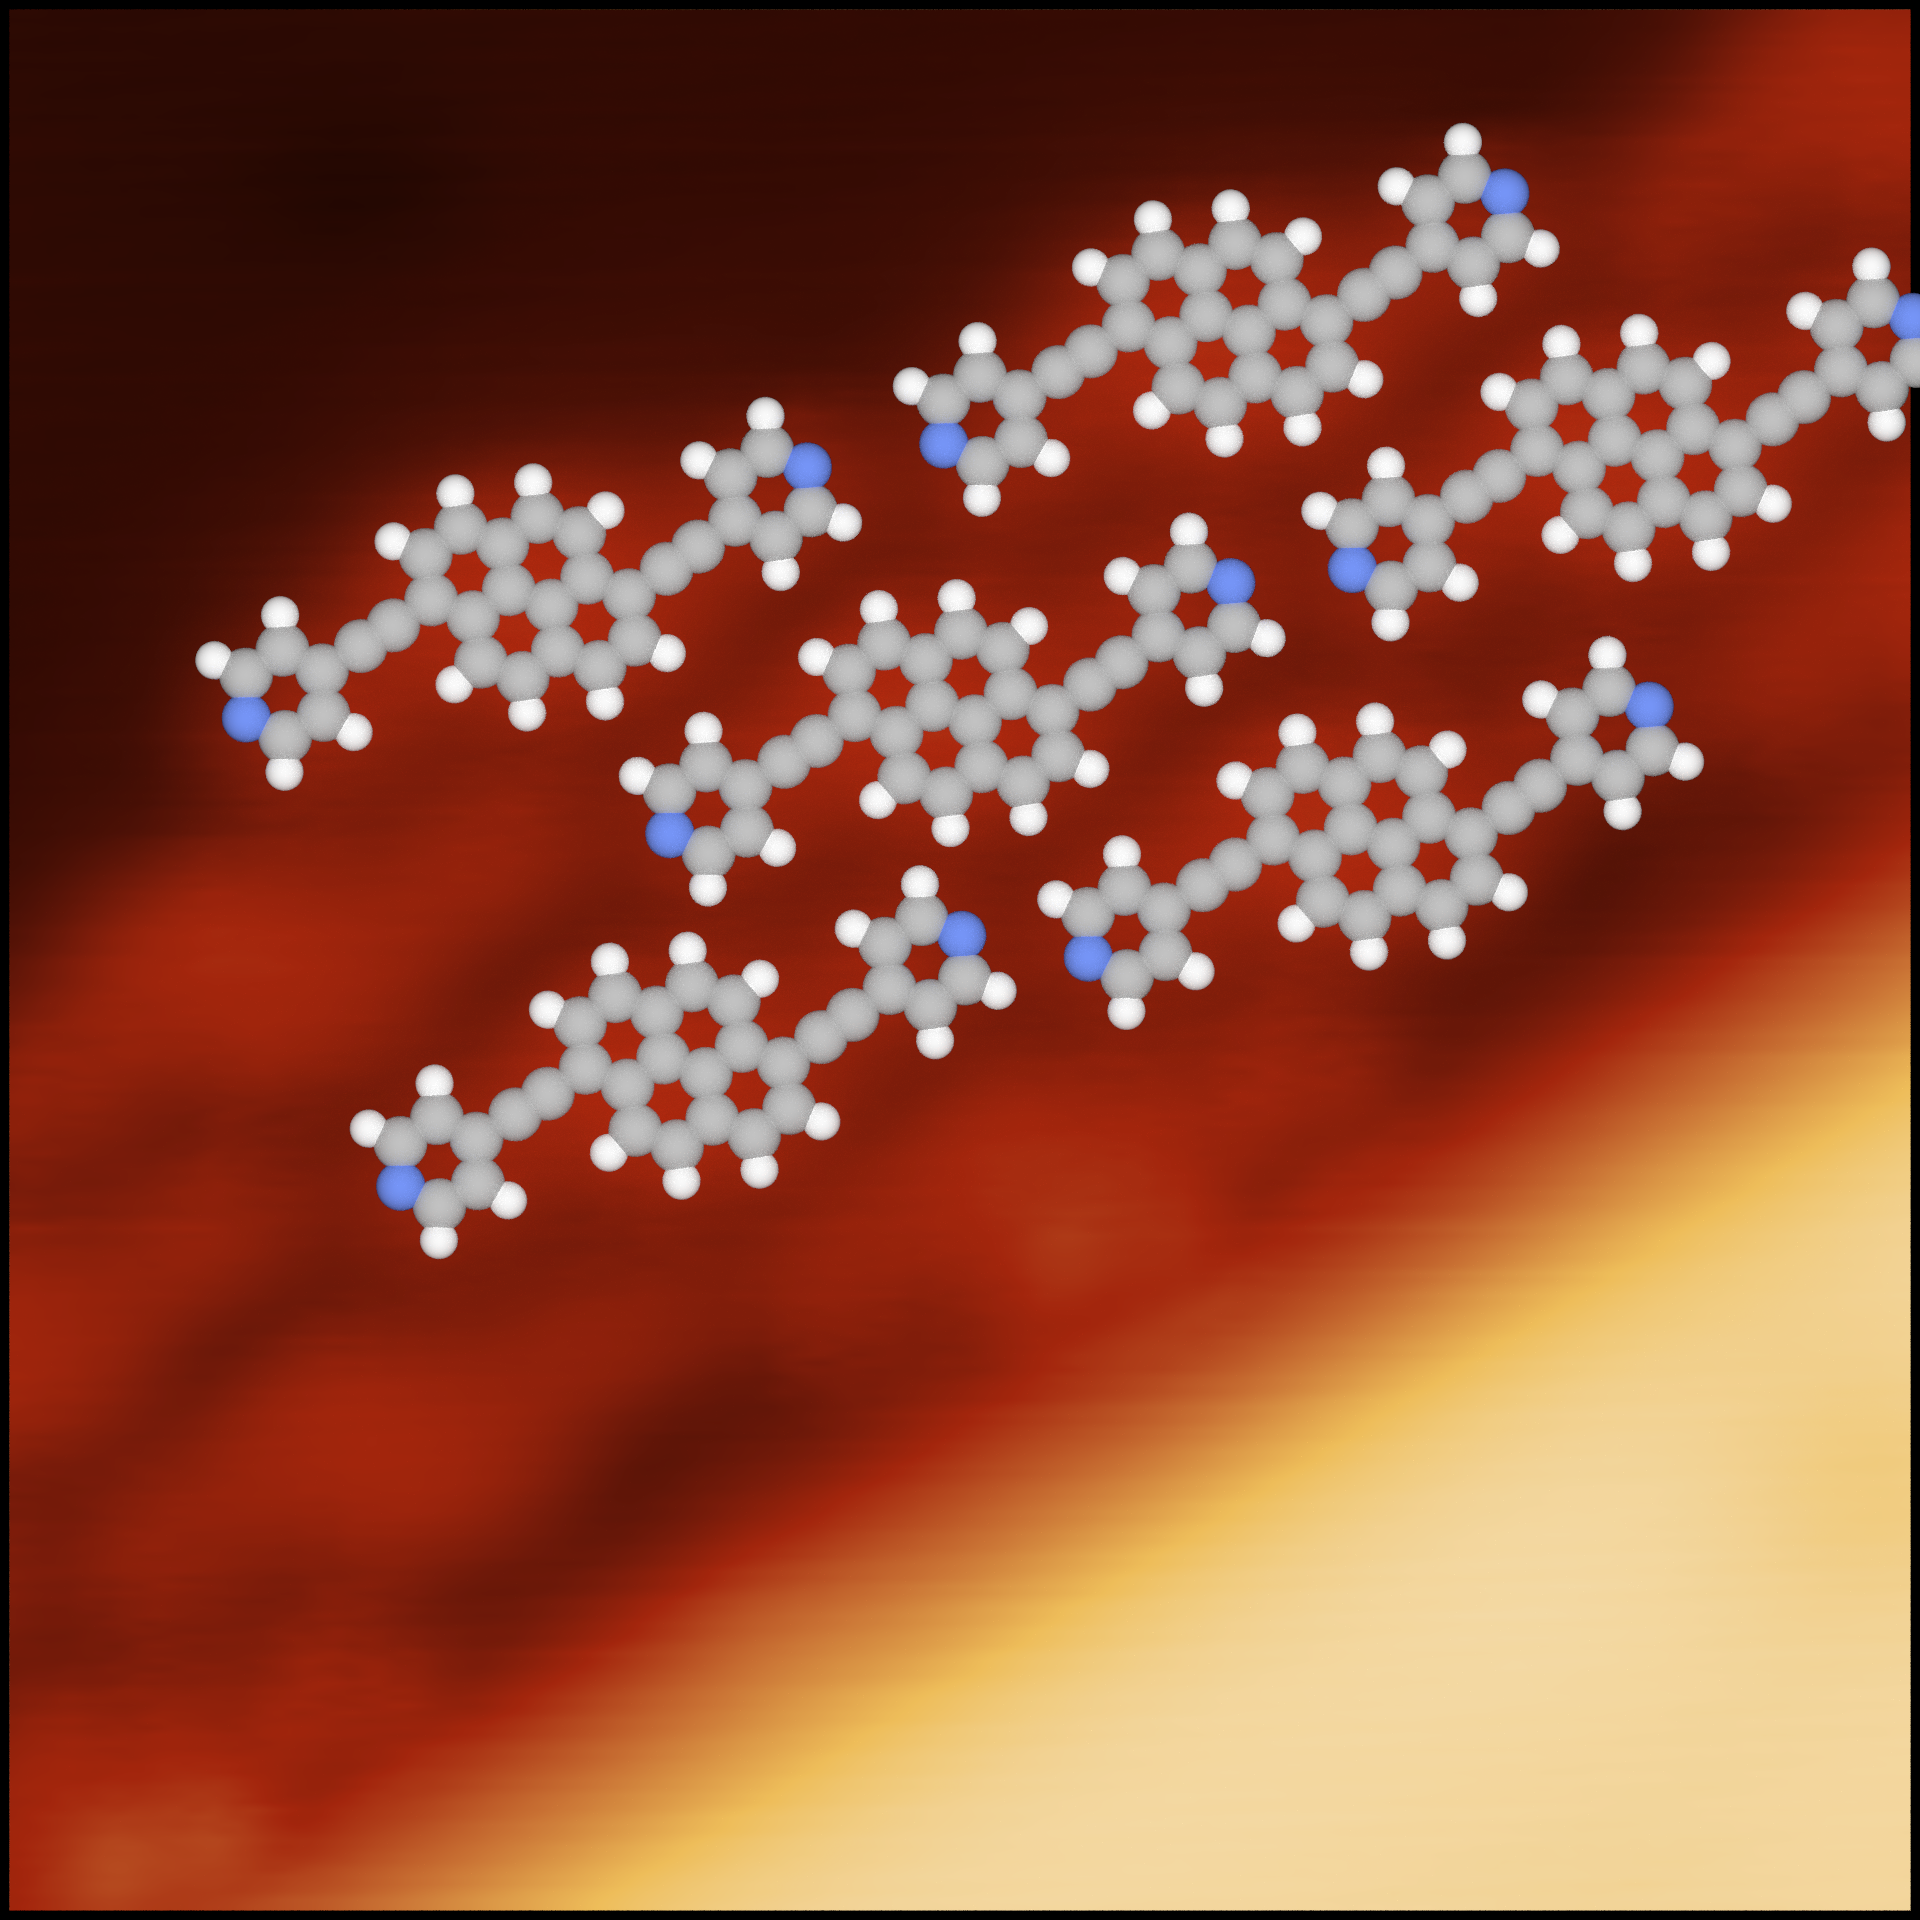
\includegraphics[width=0.45\textwidth]{./images/F160630-101110-model.png}}
  \caption{Dense packed binding motiv (upper left) and kagome-lattice coexisting on two different substrate steps. The image shows 4 different moire-periodicities (two on the lower step in the upper part of the image - two on the lower part of the image). While the growth of the molecules starts on step edges with a preferred dense-packed orientation, the main motiv remains the kagome-type of ordering.}
 \label{fig:trans-dense-packed}
\end{figure}
